\chapter{On Transformer Classifiers} \label{chapter:4}
\section{Trainability}

Having already analyzed the Transformer architecture, we will now proceed with a discussion on whether these architectures are
capable of being trained to \emph{recognize} context-free grammars. Firstly, we need to define what \emph{recognize} means in the context of our problem. In this case, we define \emph{recognition} of a string as determining whether or not the string belongs to the language in question. This is essentially a membership test: is the string a valid member of the language?

However, before we dive into this analysis on the \emph{trainability} of Transformers, which will be backed by experimental data and experiments, we
first must analyze whether these architectures are capable of learning context-free grammars or not - in essence,
are they \emph{expressive} enough to generate an internal model of a context-free grammar?

In addition to discussing the expressiveness and trainability of these models on the problem of classifying sequences on their membership to CFGs, we will also focus on explainability. By analyzing key aspects of the Transformer architecture, such as attention patterns, we aim to gain insights into the inner workings and behaviour of the model when processing and encoding the underlying structures in a CFG. Explainability is crucial, not only for improving transparency and trustworthiness of these complex models, but also for understanding the limits of their trainability and expressiveness.

Bhattamistra et al.~\cite{bhattamistra-transformers-formal-languages} prove that these architectures are expressive enough to recognize
the Shuffle-Dyck-$k$ family of languages and notes the special case of $k=1$, where Shuffle-Dyck-$k$ is equal to Dyck-1 languages.

Ströbl et al.~\cite{strobl2024formal} specify that this Transformer is one with soft-attention
(i.e.: softmax attention, as defined in Section~\ref{section:attention}) with future masking, positional encoding only, no layer normalization and no residual connections.
However, Hahn \cite{hahn-transformer} proved that hard-attention Transformers cannot model Dyck-$k$, and that soft-attention Transformers cannot model Dyck-$k$ with perfect cross entropy.

Yao et al.~\cite{bounded-hierarchical-languages} describe a Transformer with 3 layers, $\frac{i}{n}$ positional encoding, softmax attention and causal masking that should be sufficient to \emph{recognize} Dyck-$k$.

Table~\ref{table:author-experiments} presents the different architectures used by the authors.

\begin{table}[ht]
\centering
\begin{tabular}{l || c c c c c}
\toprule
\textbf{Author} & \textbf{Layers} & \textbf{Attention} & \textbf{PE} & \textbf{Masking} \\
\midrule
Bhattamistra et al. & Unspecified & Soft-Attention & Unspecified & Unspecified \\
Ströbl et al. & Unspecified & Soft-Attention & Sinusoidal & Future \\
Hahn & Unspecified & Hard-Attention & Unspecified & Unspecified \\
Yao et al. & 3 & Soft-Attention & $\frac{i}{n}$ & Causal \\
\bottomrule
\end{tabular}
\caption{Architectures used by different authors for classifying Dyck-$k$ languages with Transformers}
\label{table:author-experiments}
\end{table}


The experiments conducted and detailed below aim to validate the work done by the aforementioned authors, through experimentation.

\paragraph{Summary of experiments}
The table below shows the parameters used to configure our different models. Training hyperparameters will be discussed in a later chapter. 

\begin{table}[h!]
\centering
\begin{tabular}{c || c c c c c c c c c}
\toprule
 &$N$ & $d_{\text{model}}$ & $d_{\text{ff}}$ & $h$ & $P_{\text{drop}}$ & masking & PE & Context length & $|\Sigma|$  \\
\midrule
1 & 2 & 256 & 512 & 1 & 0.1 & bidirectional & none & 16 & 2 \\
2 & 2 & 256 & 512 & 1 & 0.1 & causal & none & 16 & 2 \\
3 & 2 & 256 & 512 & 1 & 0.1 & bidirectional & none & 16 & 6 \\
4 & 2 & 256 & 512 & 1 & 0.1 & causal & none & 16 & 6 \\
5 & 3 & 256 & 512 & 1 & 0.1 & causal & $\frac{i}{n}$ & 16 & 6 \\
6 & 2 & 256 & 384 & 1 & 0.1 & bidirectional & none & 128 & 6 \\
7 & 2 & 384 & 768 & 1 & 0.1 & bidirectional & none & 4096 & 6 \\
\bottomrule
\end{tabular}
\caption{Transformer architectural parameters}
\label{table:transformer_model_archs}
\end{table}

Here, $N$ represents the number of layers (or encoder blocks), $d_{\text{model}}$ is the embedding dimension, $d_{\text{ff}}$ is the dimension of the feed-forward network, $h$ is the number of attention heads, and $P_{\text{drop}}$ is the dropout probability \cite{dropout}. 

The masking parameter allows us to specify the type of attention mask to use, which can be either \textbf{bidirectional} or \textbf{causal} (see Section~\ref{section:attn_masks} for details). If no mask is specified, a bidirectional mask is applied by default.

The PE (positional encoding) parameter lets us choose the type of positional encoding, which can be either \textbf{absolute} or \textbf{sinusoidal}, as described in Equations \ref{eq:abs_pos_enc} and \ref{eq:sin_pos_enc}. If the PE parameter is set to \textbf{none}, no positional encoding is applied.

Context length is the maximum sequence length accepted by the model and $|\Sigma|$ is the size of our alphabet, as defined in Section~\ref{section:dyck_k}. For example, when $|\Sigma| = 2$, we are referring to a Dyck-1 language, and with $|\Sigma| = 6$, we refer to a Dyck-3 language.

These experiments were done to visualize attention patterns in a manageable way, as longer sequence lengths will only make the visualization more complex. However, we also test the \emph{trainability} of these Transformers on longer sequence lengths, as seen in Experiment 7.

As we seek to explore these attention matrices and their patterns, should they exist, we extract these matrices after training, to see whether patterns appear that can help show Transformers are able to learn Dyck-$k$ languages.

Before we jump into the analysis of attention patterns, we will first define a systematic approach for interpreting these matrices. $\text{Attn}_{m, k}(i, j)$, refers to the attention at layer $m$, (attention) head $k$ of $\verb|tok[|i\verb|]|$ with respect to $\verb|tok[|j\verb|]|$, where $\verb|tok[|i\verb|]|$  and $\verb|tok[|j\verb|]|$ are the tokens at position $i$ and $j$, respectively. Furthermore, $\text{Attn}_{m, k}(i)$ or the attention of $\verb|tok[|i\verb|]|$ with respect to the sequence, refers to row $i$ in the attention matrix for layer $m$, head $k$.

Also, we find it important to note that all attention matrices shown below are min-max normalized to the range $[-1, +1]$, for easier visualization of attention scores.



\subsection{Experiments on Dyck-1 Classifier Transformers}

We will now describe the experiments conducted with two Transformers built to classify Dyck-1 languages - these correspond to the first 2 experiments in Table~\ref{table:transformer_model_archs}.

\subsubsection{Bidirectionally masked Transformer} \label{subsubsection:bidirectional-dyck-1}
Figure~\ref{fig:bidirectional-dyck-1} shows two examples of attention matrices for the Transformer corresponding to the first experiment in Table~\ref{table:transformer_model_archs}, trained on Dyck-1 samples that achieved perfect (i.e.: 100\%) accuracy over train, validation and test datasets, as well as a near-zero loss.

\begin{figure}[h]
    \centering
    \begin{subfigure}{.5\textwidth}
      \centering
      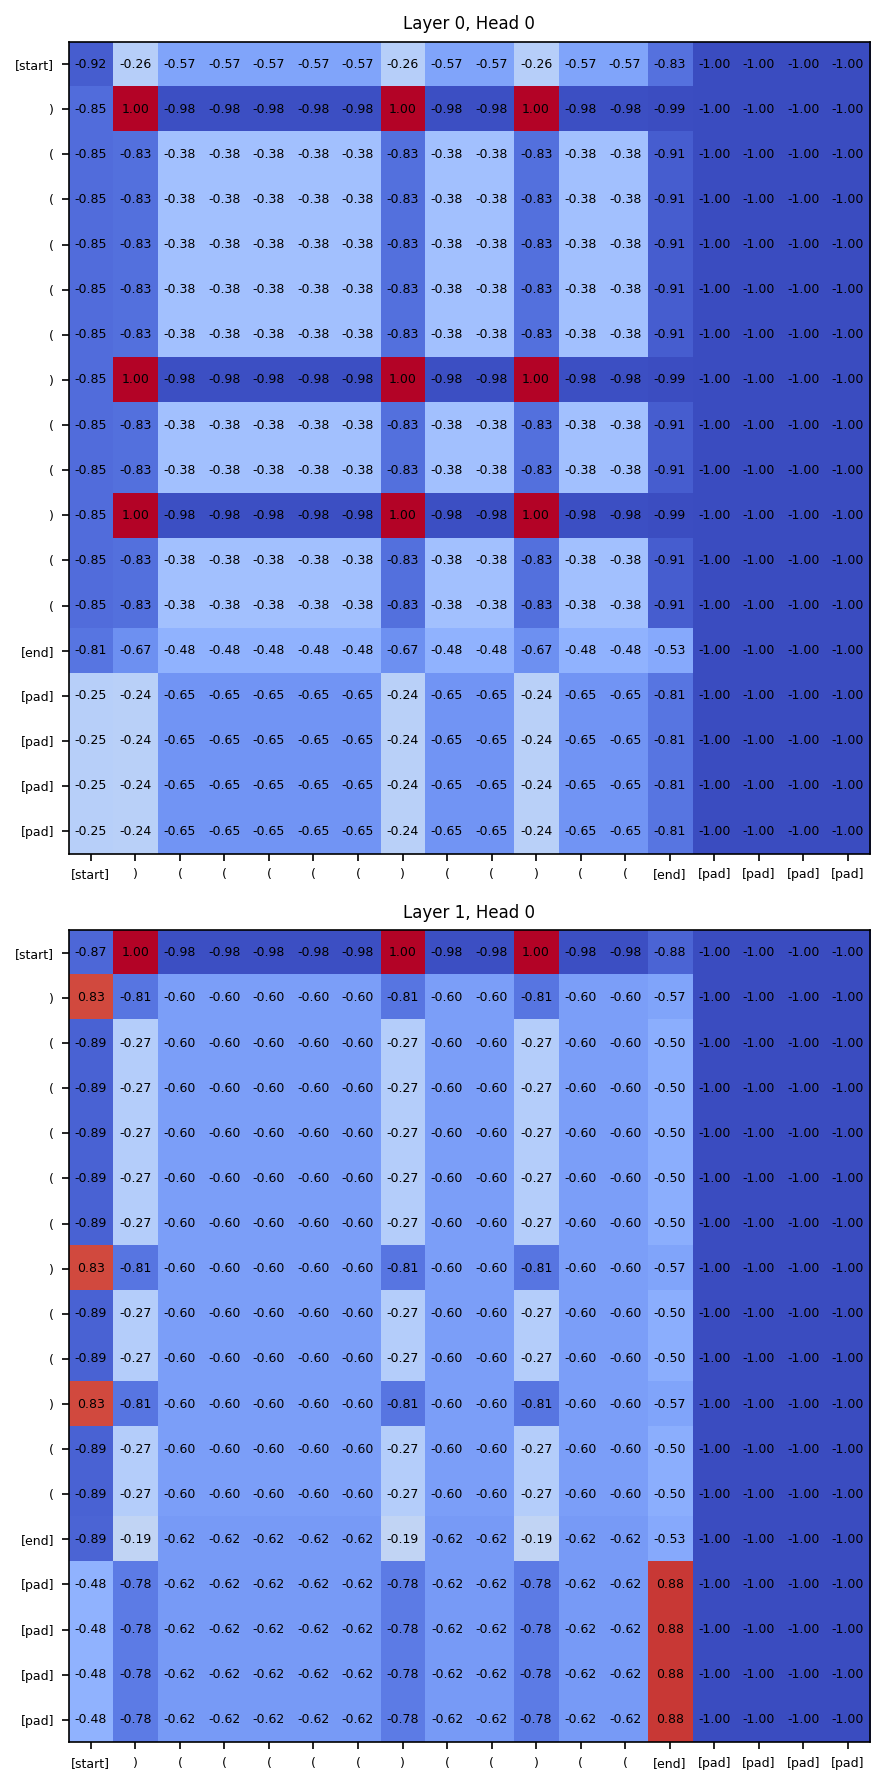
\includegraphics[width=.8\linewidth]{docs/figs/dyck_1/sequence_1_dyck_1.png}
      \caption{Attention matrices of string \\ $s \notin \text{Dyck}-1$}
      \label{fig:neg-dyck-1}
    \end{subfigure}%
    \begin{subfigure}{.5\textwidth}
      \centering
      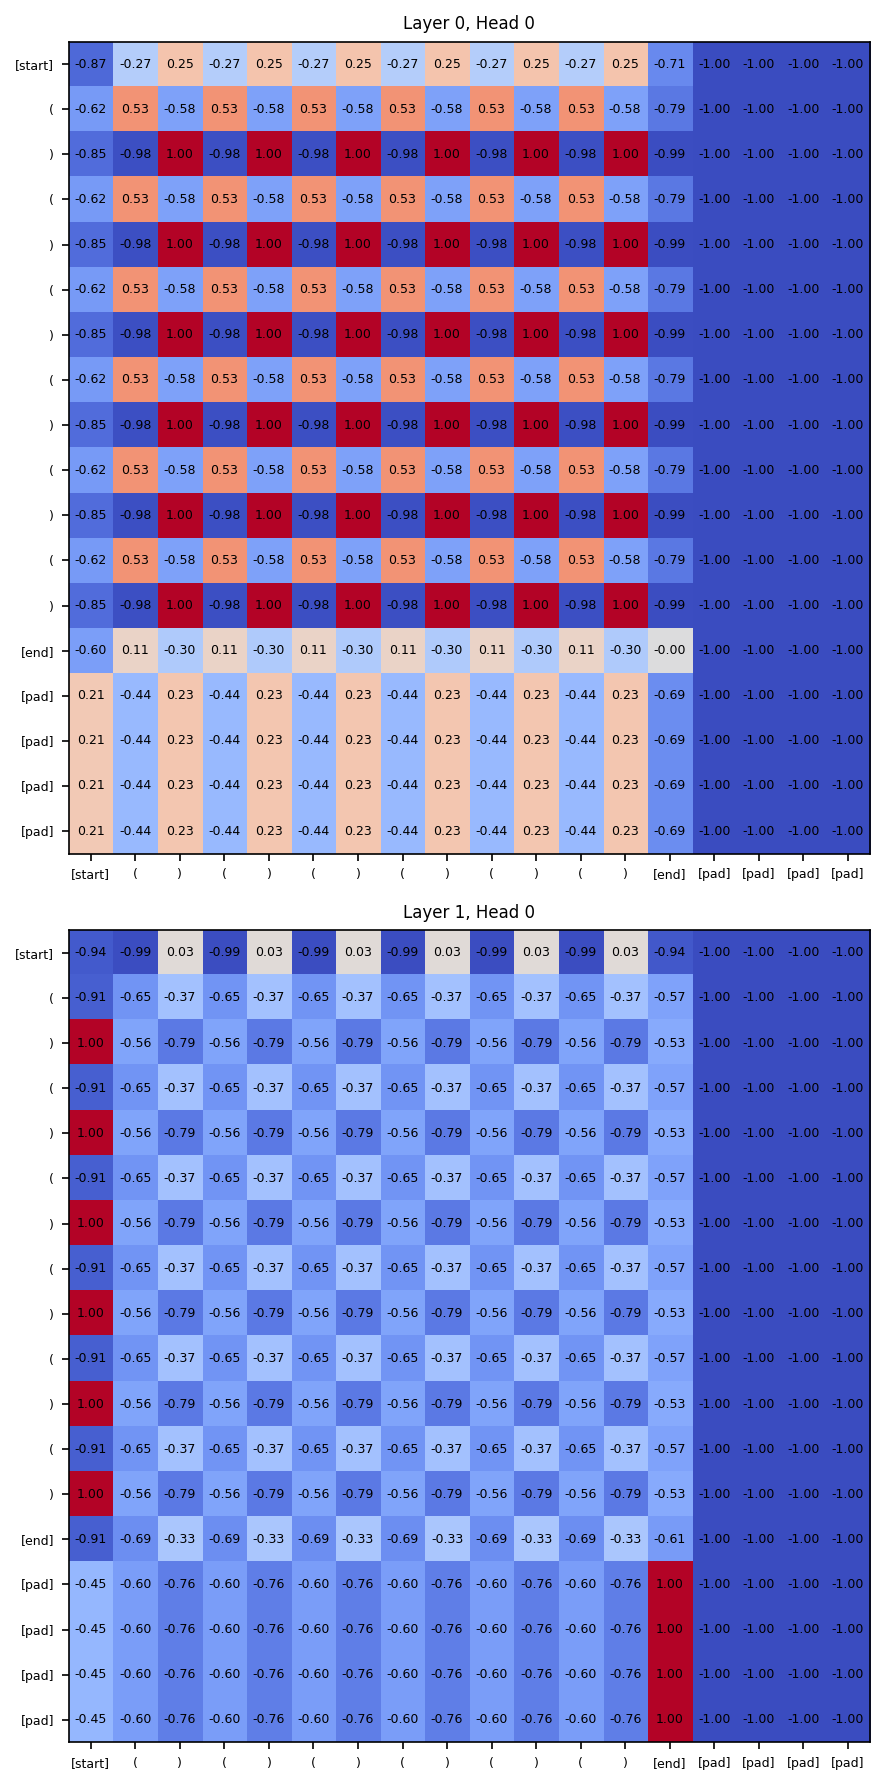
\includegraphics[width=.8\linewidth]{docs/figs/dyck_1/sequence_4_dyck_1.png}
      \caption{Attention matrices of string \\ $s \in \text{Dyck}-1$}
      \label{fig:pos-dyck-1}
    \end{subfigure}
    \caption{Attention matrices of a Transformer with a pad-token mask trained on Dyck-1 strings}
    \label{fig:bidirectional-dyck-1}
\end{figure}

Both sets of attention matrices display a distinct and meaningful pattern, illustrating how certain tokens attend more strongly to specific others, which aligns with the structure of the Dyck-1 language. Specifically, looking at Figure~\ref{fig:pos-dyck-1}, we observe that in Layer 0, the first opening bracket (`\verb|(|') primarily attends to the other opening brackets in the sequence. This suggests that the model has learned to recognize the structural importance of matching opening brackets, as it assigns greater attention weight to those tokens. Importantly, these opening brackets are largely ignoring the closing brackets, which indicates the model is distinguishing between different types of parentheses.

Similarly, the first closing bracket (`\verb|)|') also exhibits a strong attention pattern by attending more prominently to the other closing brackets in the sequence, but not to the opening brackets. This consistent and structured behavior in Layer 0 highlights the model's understanding of grouping similar tokens, which reflects how it is capturing the hierarchical nature of Dyck-1, where brackets must be correctly matched and nested.

However, in Layer 1, the attention pattern undergoes a transformation. Here, the first opening bracket now attends more strongly to the closing brackets, suggesting that the model in this layer has begun learning the relationships necessary for pairing open and close brackets. The first closing bracket, on the other hand, shifts its focus to attend to the opening brackets in the sequence. This inversion of attention patterns in Layer 1 may reflect the model's mechanism for resolving bracket pairs, ensuring that each opening parenthesis finds its corresponding closing counterpart.

This progressive change across layers demonstrates how the transformer is leveraging the attention mechanism to first group similar tokens (Layer 0) and then to learn the associations between these groups (Layer 1), effectively capturing the hierarchical and nested structure of Dyck-1 sequences. This process mirrors the parsing of formal languages, where early stages (lower layers) establish syntactical groupings, while later stages (higher layers) work toward resolving more complex relationships like matching parentheses.

This clear attention pattern is a key factor in the model’s ability to achieve perfect accuracy across the train, validation, and test datasets. It highlights how transformers can efficiently learn and represent formal languages by leveraging attention mechanisms across layers to capture both token-level similarities and dependencies across a sequence.

\subsubsection{Causally masked Transformer} \label{subsubsection:causal-dyck-1}
However, if we take a look at the attention matrices generated by the second experiment in Table~\ref{table:transformer_model_archs}, we will see that no clear pattern is generated, as can be seen in Figure~\ref{fig:causal-dyck-1}.

In this case, the model can only ``see'' or attend to tokens behind the current token position. A causal attention mechanism restricts the model to attend only to tokens that have already been processed, avoiding future token information during the current position's attention computation, as defined in Section~\ref{section:attn_masks}.

\begin{figure}[h]
    \centering
    \begin{subfigure}{.5\textwidth}
      \centering
      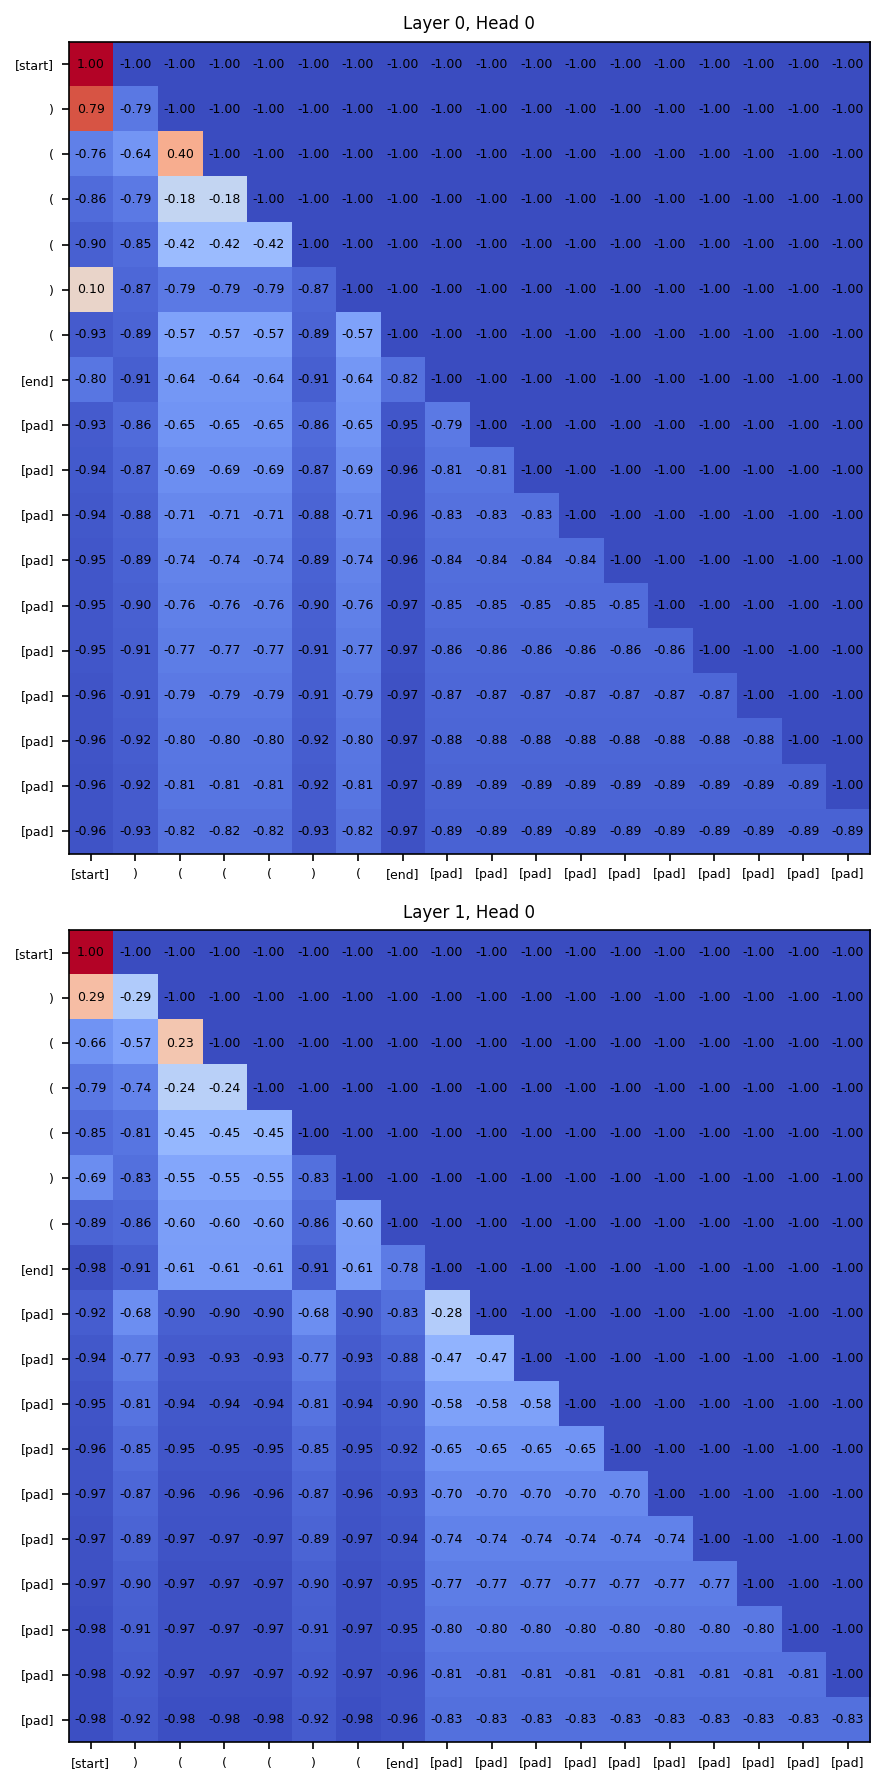
\includegraphics[width=.8\linewidth]{docs/figs/dyck_1/causal_seq_1_dyck_1.png}
      \caption{Attention matrices of string \\ $s \notin \text{Dyck}-1$}
      \label{fig:neg-causal-dyck-1}
    \end{subfigure}%
    \begin{subfigure}{.5\textwidth}
      \centering
      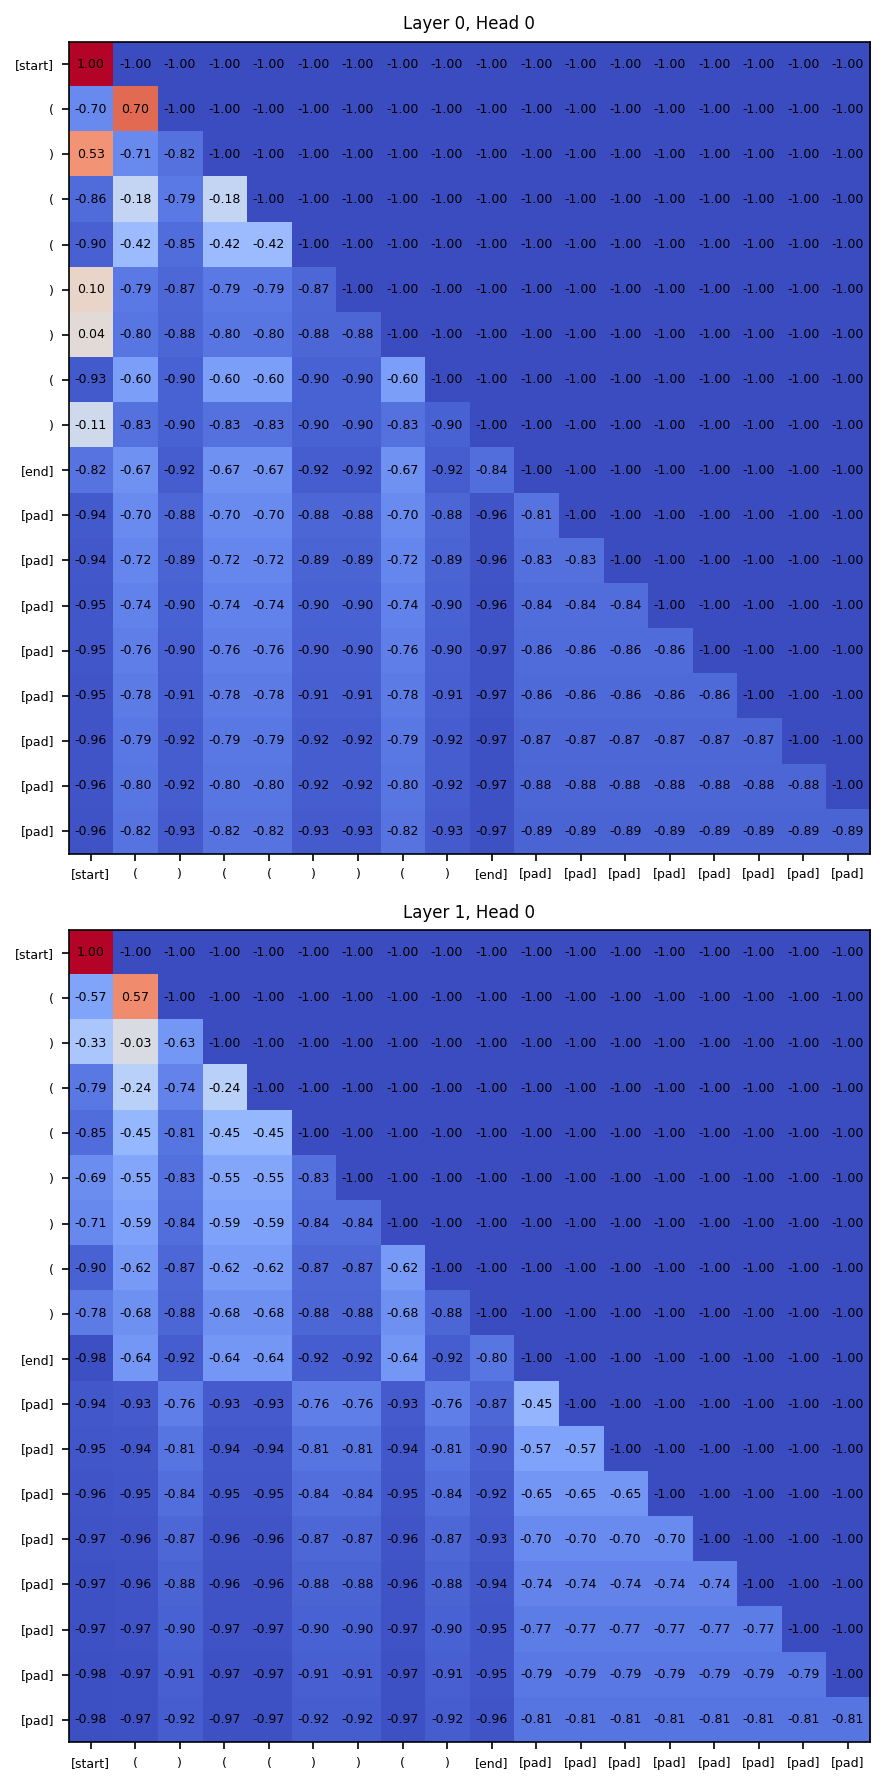
\includegraphics[width=.8\linewidth]{docs/figs/dyck_1/causal_seq_2_dyck_1.png}
      \caption{Attention matrices of string \\ $s \in \text{Dyck}-1$}
      \label{fig:pos-causal-dyck-1}
    \end{subfigure}
    \caption{Attention matrices of a Transformer with a causal mask trained on Dyck-1 strings}
    \label{fig:causal-dyck-1}
\end{figure}

Figure~\ref{fig:causal-dyck-1} shows this limitation leads to less defined attention patterns compared to the first experiment. In Layer 0, Head 0, for instance, the model primarily attends to nearby tokens in the sequence, but with little variation in attention strength. This could indicate that the model is not learning significant dependencies between tokens, or it is being overly biased by the causal restriction, preventing it from fully capturing the structure of the input sequence, such as matching parentheses.

This effect is more pronounced in deeper layers. In Layer 1, Head 0, the attention values are also spread more diffusely, and while some tokens show slightly stronger attention, the general trend reflects a failure to learn structured dependencies, as seen in the minimal variation between attention weights. Furthermore, as we traverse the sequence, attention scores become lower, showing that there is a less of a learned dependency between opening and closing brackets, which is a key part of learning to recognize Dyck-$k$ sequences.

Moreover, there is no distinct pattern like the one observed in the first experiment (refer to Table~\ref{table:transformer_model_archs}) where the model learned the dependency structure between opening and closing parentheses more clearly. This lack of a pattern in the attention matrices implies that the model may be struggling with generalizing the Dyck-1 rules, which we attribute to the causal restriction in the attention mechanism.

In this experiment, we never reached an accuracy higher than $\approx$ 60\% across the train, validation and test datasets. Furthermore, the loss across training, validation and evaluation seemed to increase, rather than decrease, as we will see in Section~\ref{section:hyperparameters-metrics}.

In summary, the causal limitation imposed in this second experiment seems to significantly impact the model’s ability to learn the intricate patterns required for Dyck-1 language parsing. While the model does attend to previous tokens, the attention matrices do not show the clear patterns needed for correctly pairing parentheses, unlike in the first experiment. This leads to the conclusion, supported by the low training and test accuracies, that causal attention alone may not be sufficient for creating Transformers trainable enough to generalize certain formal languages from limited samples, especially when bidirectional dependencies are crucial, as is the case with Dyck-1.

\subsection{Experiments on Dyck-3 Classifier Transformers}

We will now describe the experiments conducted with Transformers built to classify Dyck-3 languages - these correspond to the third, fourth and fifth experiments in Table~\ref{table:transformer_model_archs}.

\subsubsection{Bidirectionally masked Transformer}
In these experiments, both sets of attention matrices display meaningful patterns, which illustrates how certain tokens in the sequence attend more strongly to specific others, in this case aligning with the structure of the Dyck-3 language. 

Albeit not as clear as the patterns in the experiments done with Dyck-1 languages, similar behaviours can be seen in these matrices. This decrease in the clarity of the pattern in the attention matrices was expected as the language became much more complex, however, the Transformer still managed to classify all sequences belonging to the language perfectly across train, validation and test datasets, reaching an accuracy of 100\%, with a near-zero loss.

\begin{figure}[h]
    \centering
    \begin{subfigure}{.5\textwidth}
      \centering
      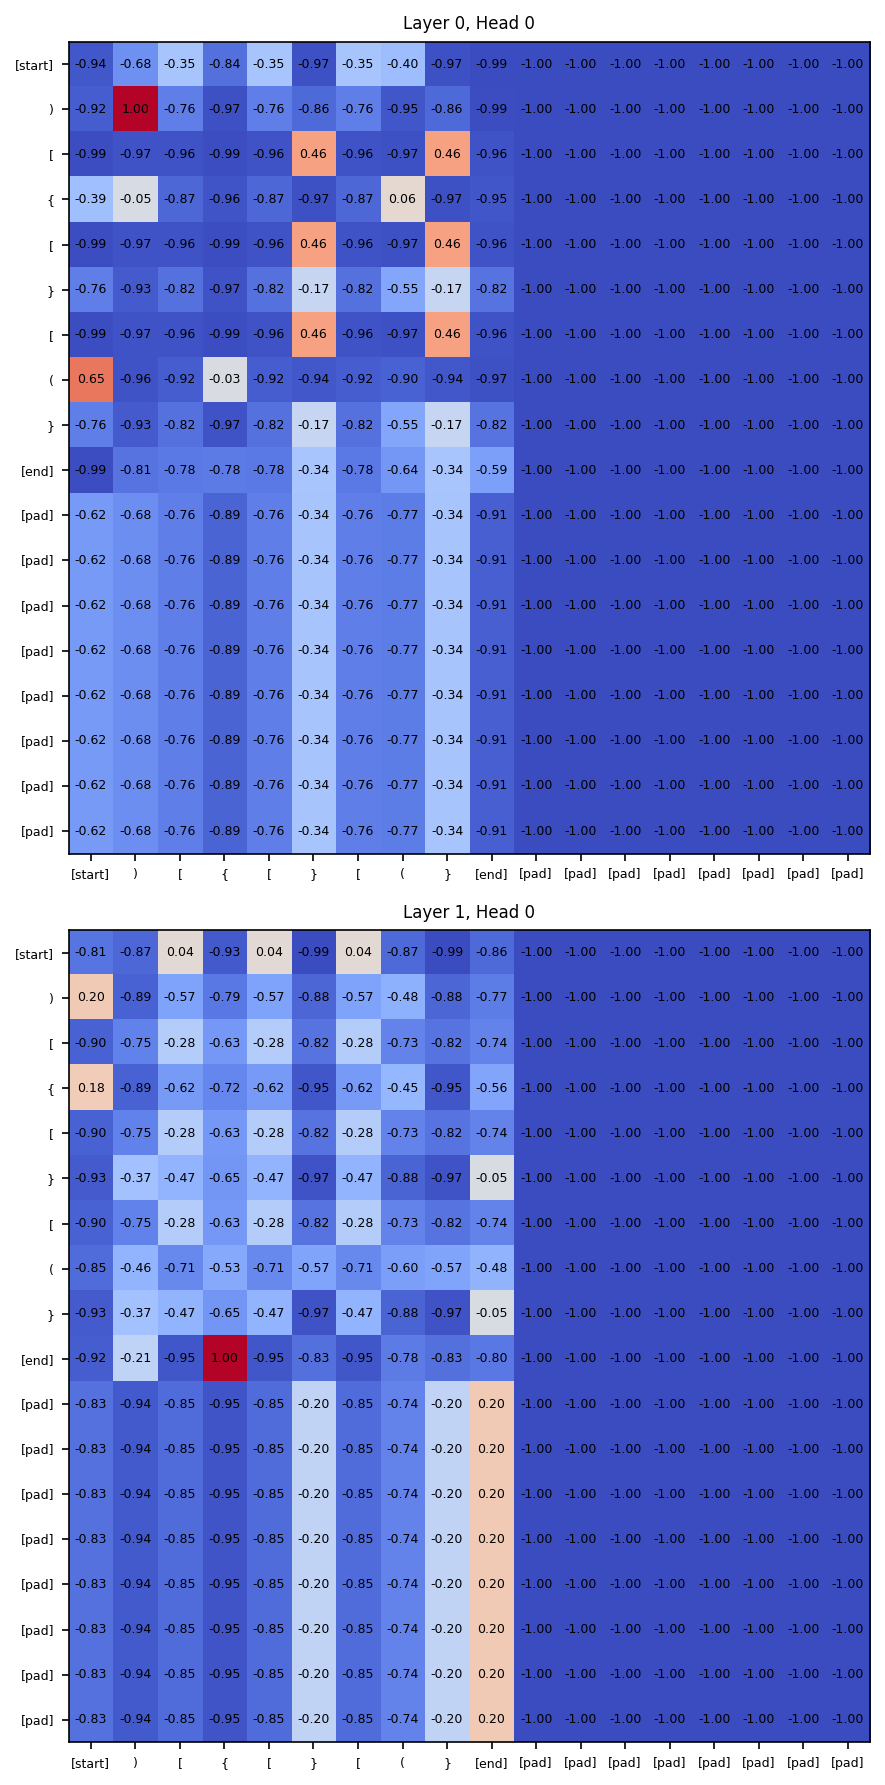
\includegraphics[width=.8\linewidth]{docs/figs/dyck_3/pad_tok_seq_1_dyck_3.png}
      \caption{Attention matrices of string \\ $s \notin \text{Dyck}-3$}
      \label{fig:neg-dyck-3}
    \end{subfigure}%
    \begin{subfigure}{.5\textwidth}
      \centering
      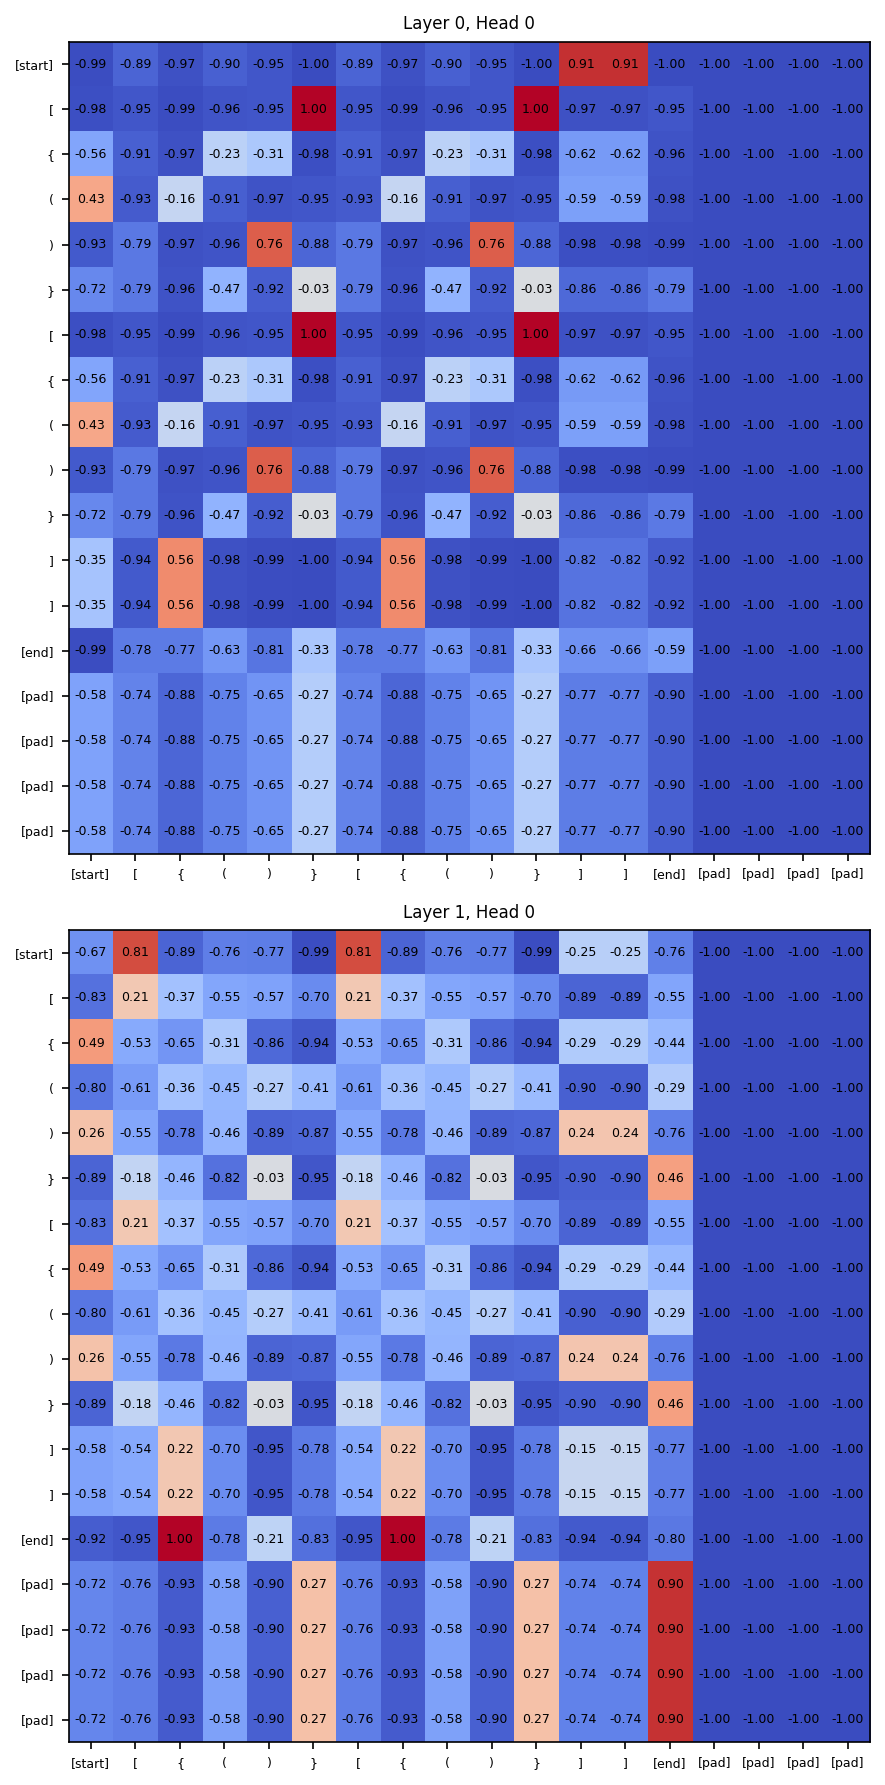
\includegraphics[width=.8\linewidth]{docs/figs/dyck_3/pad_tok_seq_2_dyck_3.png}
      \caption{Attention matrices of string \\ $s \in \text{Dyck}-3$}
      \label{fig:pos-dyck-3}
    \end{subfigure}
    \caption{Attention matrices of a Transformer with a pad-token mask trained on Dyck-3 strings}
    \label{fig:bidirectional-dyck-3}
\end{figure}

Even though these matrices do not have a pattern as clear as those in Figure~\ref{fig:bidirectional-dyck-1}, we still can see elements that indicate the Transformer has learned relations between tokens in the sequences. For example, if we look at Figure~\ref{fig:bidirectional-dyck-3}, the attention values of specific tokens are repeated throughout the matrix. Let us look at the attention values of the following token pairs in Layer 0, Head 0 in Figure~\ref{fig:pos-dyck-3}, where

\begin{equation}\label{eq:repeated_attn_vals}
    \text{Attn}_{0,0}(\verb|(|, \verb|{|_1) = \text{Attn}_{0,0}(\verb|(|, \verb|{|_2) = -0.16
\end{equation}

Equation~\ref{eq:repeated_attn_vals} shows that the attention of the first opening parentheses with the opening curly braces in the sequence is the same, showing a pattern where tokens are attended to with the same importance throughout the sequence. This is repeated for other tokens as well, such as

\begin{equation}\label{eq:repeated_attn_vals_2}
    \text{Attn}_{0,0}(\verb|[|, \verb|[|_1) = \text{Attn}_{0,0}(\verb|[|, \verb|[|_2) = 0.21
\end{equation}

Equation~\ref{eq:repeated_attn_vals_2} shows that the attention of the first opening square bracket with respect to the other opening square brackets in the sequence shown in \ref{fig:pos-dyck-3} is a constant value.

From these results, we can hypothesize that even for more complex languages such as Dyck-3, the bidirectional attention mechanism is capable of effectively capturing the hierarchical dependencies and structures present in these languages.

\subsubsection{Causally masked Transformer}

Once more, when the Transformer is trained with a causal mask rather than a bidirectional one, we find that not only the patterns in the attention matrices are lost, but also the model does not achieve generalization and near-perfect performance over the data. For Dyck-3 sequences, we found the effect of the mask to be even more pronounced, with variations of attention scores dropping drastically with the token position, in essence, ``losing'' information on whether the string up to that point was balanced or not. 

\begin{figure}[h]
    \centering
    \begin{subfigure}{.5\textwidth}
      \centering
      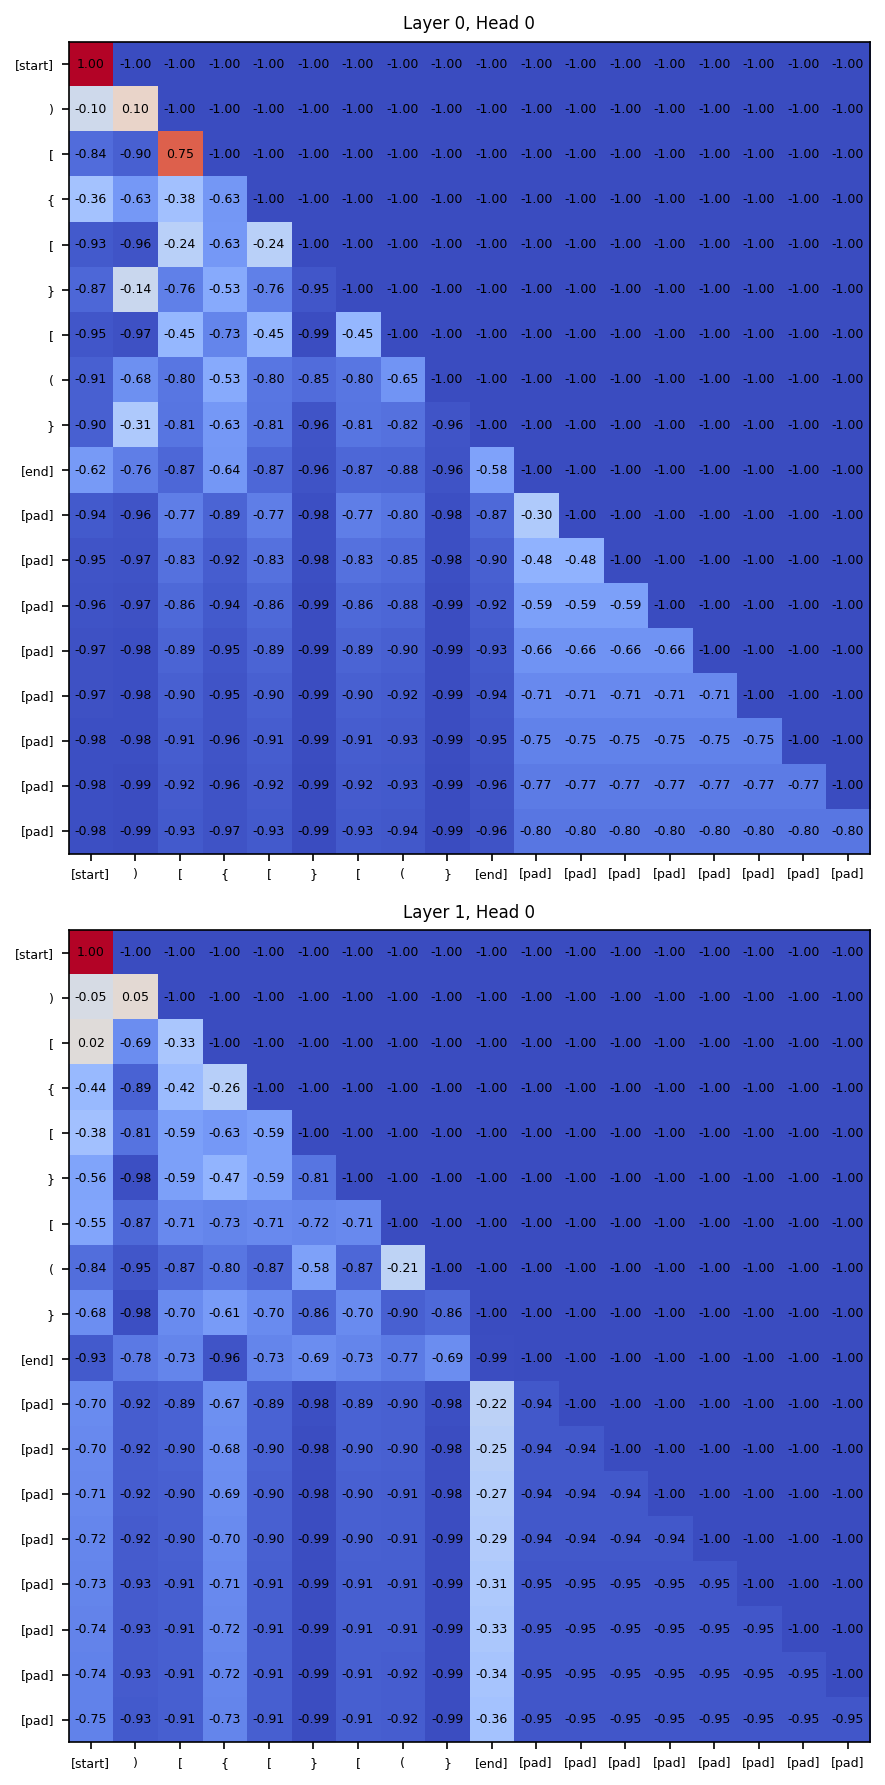
\includegraphics[width=.8\linewidth]{docs/figs/dyck_3/causal_seq_1_dyck_3.png}
      \caption{Attention matrices of string \\ $s \notin \text{Dyck}-3$}
      \label{fig:neg-causal-dyck-3}
    \end{subfigure}%
    \begin{subfigure}{.5\textwidth}
      \centering
      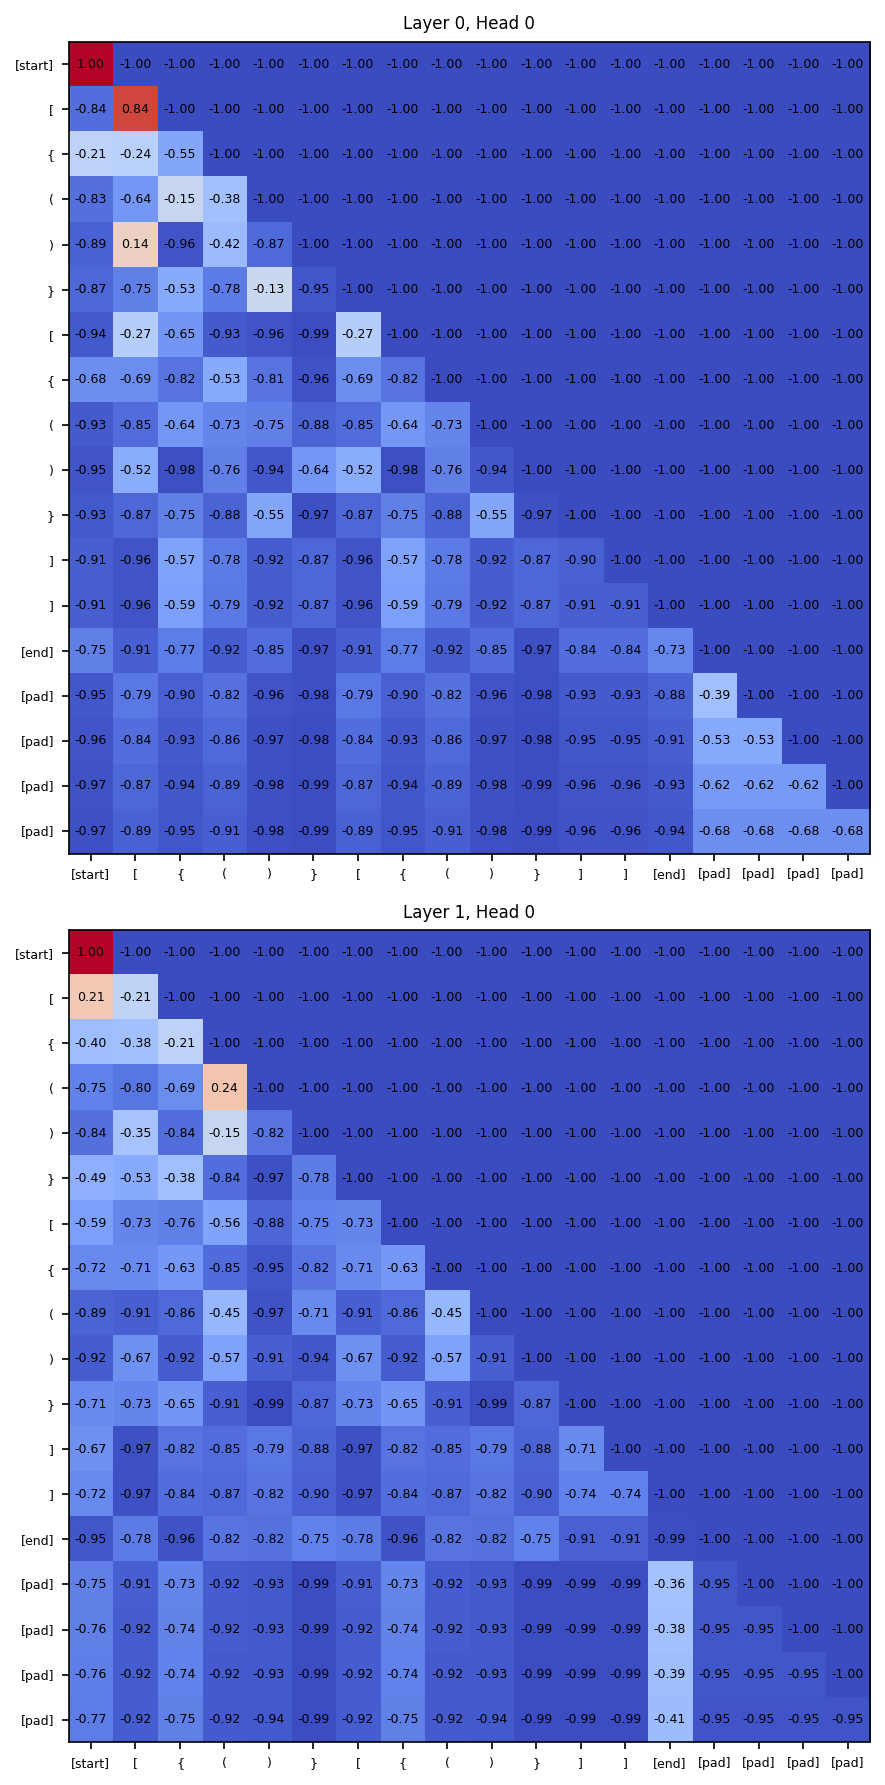
\includegraphics[width=.8\linewidth]{docs/figs/dyck_3/causal_seq_2_dyck_3.png}
      \caption{Attention matrices of string \\ $s \in \text{Dyck}-3$}
      \label{fig:pos-causal-dyck-3}
    \end{subfigure}
    \caption{Attention matrices of a Transformer with a causal mask trained on Dyck-3 strings}
    \label{fig:causal-dyck-3}
\end{figure}

Let us look at Figure~\ref{fig:pos-causal-dyck-3}, more specifically at Layer 0, Head 0, where attention values at the start of the sequence are much higher than attention values at the end of the sequence, where they tend to be much nearer the (normalized) minimum value of $-1$. For example, if we consider the attention of the first token with respect to itself, we see a much higher attention value: 

\begin{equation}
    \text{Attn}_{0, 0}(\verb|[|, \verb|[|) = 0.84
\end{equation}

However, if we consider tokens towards the end of the word, such as the attention of the last token with respect to itself, we see it is much lower, and does not follow the pattern seen in bidirectionally masked Transformers:

\begin{equation}
    \text{Attn}_{0, 0}(\verb|]|, \verb|]|) = -0.91
\end{equation}

We attribute this to the causal restriction imposed by the mask, which limits the ability of the model to ``see'', generate internal pairings between brackets, and thus train and generalize to recognize Dyck-3 strings from limited samples.

\subsection{Out-of-distribution experiments} \label{subsection:ood-experiment}

In this experiment, we investigate whether Transformer classifiers can maintain their accuracy when processing sequences longer than those they were trained on.

We trained a 2-layer Transformer model with soft attention, no positional encoding, and bidirectional masking on sequences from the Dyck-3 language. Our previous results already showed this model can generalize well, achieving perfect classification of the Dyck-3 language with a limited number of training samples. The training sequences had lengths ranging from 0 to 96 tokens. As shown in Table \ref{table:transformer_model_archs}, the model’s context window was set to 128 tokens, meaning it was theoretically capable of handling sequences up to 128 tokens in length. During training, the model quickly reached 100\% accuracy and near-zero loss, which is consistent with the results observed in previous experiments.

For evaluation, we used a different dataset containing Dyck-3 sequences with lengths ranging from 32 to 128 tokens. Given the model’s (near) perfect performance on both the training and validation sets, we expected it to perform well on the test dataset. However, the model only achieved an accuracy of $\approx 75\%$. We can visualize this in Figure~\ref{fig:ood_results}.

\begin{figure}[ht]
    \centering
    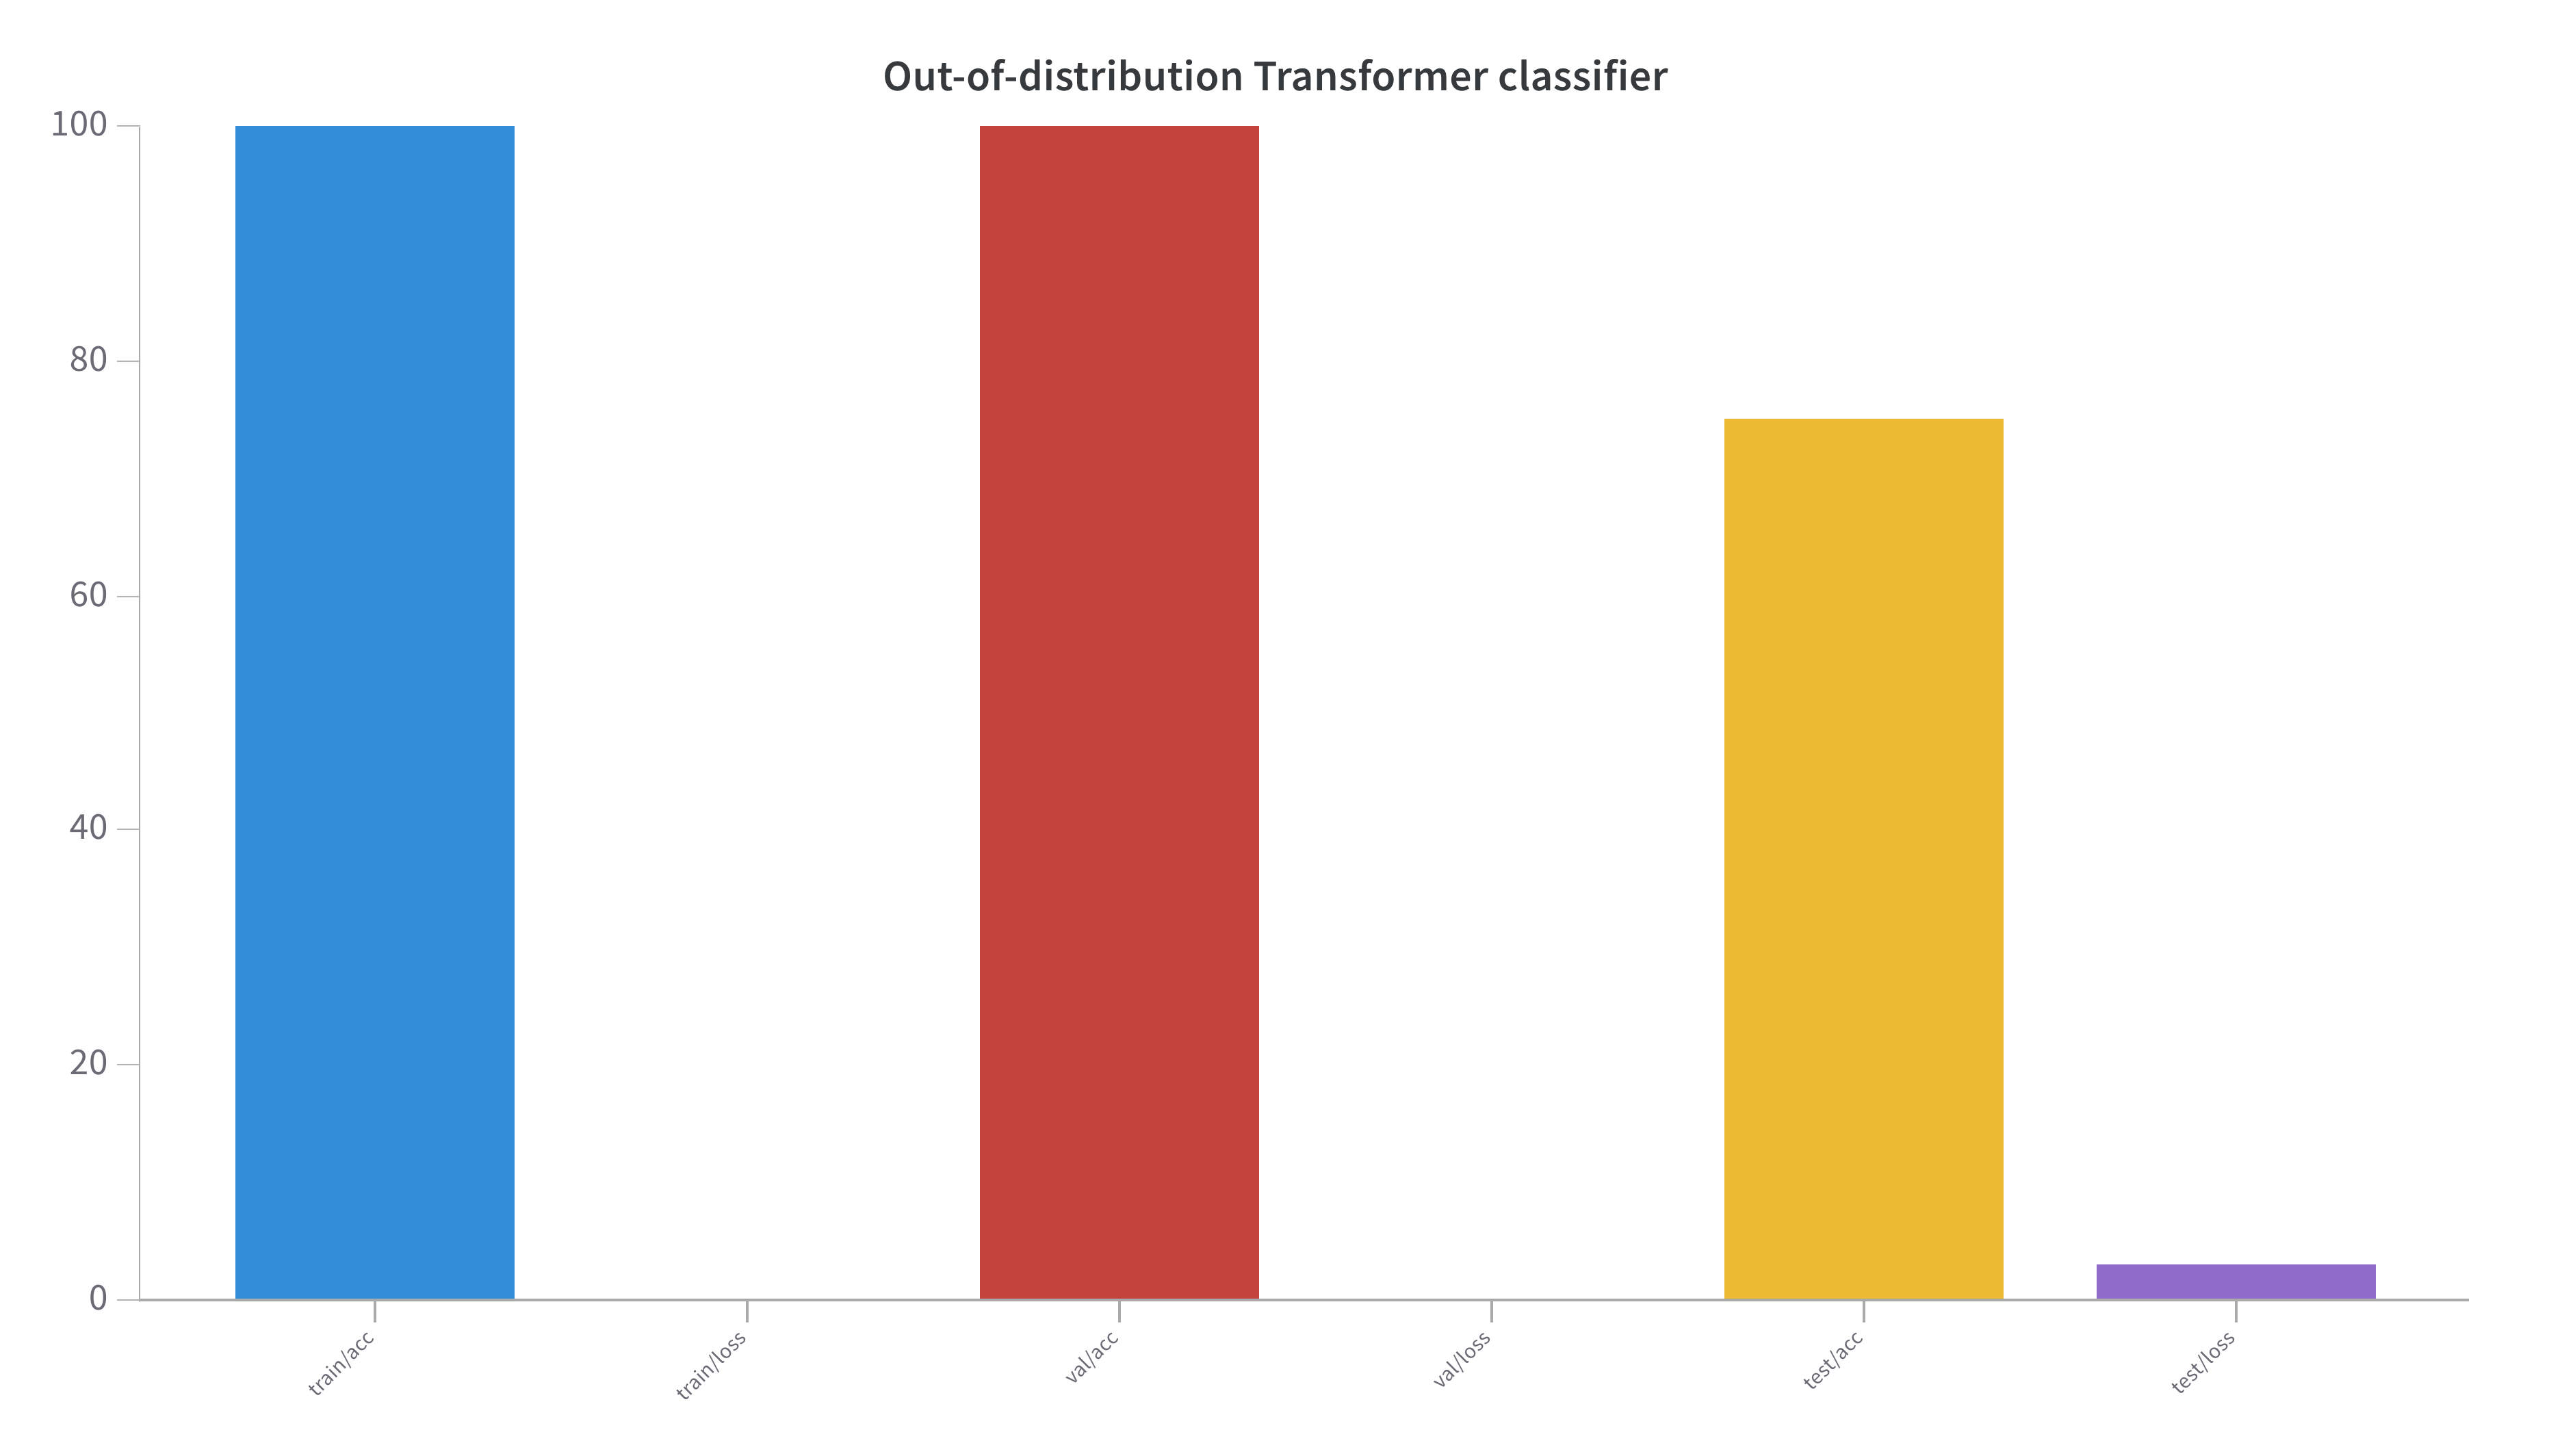
\includegraphics[width=0.8\linewidth]{docs/figs/ood_results.png}
    \caption{Accuracy/Loss for Out-of-distribution Transformer classifier}
    \label{fig:ood_results}
\end{figure}

This outcome suggests that the model struggles with sequences longer than 96 tokens, despite having a larger context window of 128 tokens. Since $\approx 75\%$ accuracy could correspond to correctly classifying test sequences up to 96 tokens long, assuming a uniform distribution of sequence lengths, we hypothesize that Transformer models can only effectively process sequences up to the maximum length they were trained on, even if their context window supports longer sequences. 

Therefore, we found an important limitation of these models, since even though Transformers can generalize across different sequence lengths, their ability to classify sequences accurately is bounded by the lengths present in the training data. In essence, for the model to perform well on longer sequences, the training dataset must include samples that cover the full range of sequence lengths up to the desired maximum.

\subsection{Long-context Transformer experiments}

In our final experiment, we aimed to assess whether these models could accurately classify longer Dyck-3 strings, testing their ability to handle significantly longer sequences. We conducted this experiment using sequences ranging in length from 0 to 4096, which allowed us to push the boundaries of sequence length beyond what had been tested in previous experiments. The model we used was a 2-layer Transformer with soft attention, no positional encoding, and bidirectional masking, as in earlier setups.

The model demonstrated rapid learning, achieving an accuracy of 100\% and a near-zero loss in a short amount of time, similar to our previous experiments. This quick convergence suggests that Transformer models do not struggle with recognizing Dyck-$k$ strings, even as sequence lengths increase significantly. In fact, sequence length does not appear to pose a challenge, as long as the sequences fall within the range of lengths seen during training.

These results indicate that the model's architecture, particularly its use of bidirectional masking and soft attention, is well-suited to the task of Dyck string classification, handling long sequences just as effectively as shorter ones.

Due to the sheer size and complexity of the attention matrices, which in this experiment are $4096 \times 4096$, we found it nigh impossible to visualize any meaningful attention patterns. The vast amount of information stored in these matrices makes it extremely difficult to interpret or identify specific trends or behaviors within the attention mechanism. Each matrix element represents the attention weight between every pair of tokens in the sequence, leading to over 16 million individual data points per matrix.

As a result, the scale of the data makes visual inspection nearly impossible, and even traditional visualization techniques, such as the heatmaps used in previous experiments, become ineffective due to the dense and intricate nature of the attention distribution. This highlights one of the limitations of working with very long sequences in Transformer models, where the complexity of the attention mechanism grows quadratically with sequence length, making it increasingly harder to analyze and understand the model’s internal workings as the sequence length increases.

\subsection{General observations}

In our experiments, we found that while the Transformer architecture described by Ströbl et al.~\cite{strobl2024formal} is theoretically expressive enough to recognize this family of languages, it may lack sufficient trainability. 

However, a Transformer composed by 2 encoder layers (or blocks) with soft attention, pad-token masking, no positional encoding, layer normalization, and residual connections proved to be consistently trainable enough to not only recognize but also generalize effectively to both the training and test datasets. This modified architecture achieved 100\% accuracy and a loss of 0 on both sets, at least for sequences of a given length, for Dyck-$k$ languages (with different values of$k$). 

This corresponds with results achieved by Yao et al.~\cite{bounded-hierarchical-languages}, in which they empirically found Transformers are able to \emph{learn} (through training) and achieve good performance on finite samples of these languages. This highlights the difference between \emph{expressivity} and \emph{trainability}. 

However, when trying to train the model described by the authors (which corresponds to Experiment 5 in Table~\ref{table:transformer_model_archs}), we found that it does not generalize from limited samples, but instead falls into the same pitfalls our causally masked Transformers (Experiments 2 and 4) had during training, where none could surpass an accuracy of $\approx 60\%$.

It is of interest to note that we did observe some examples where a Transformer with only 1 encoder block (or layer), with the aforementioned components, was able to be trained to recognize the training and testing dataset with 100\% accuracy, however, these results were sporadic and not consistently reproducible over multiple runs.

\section{Explainability and Interpretability}

With regards to the explainability of Transformers, we have already discussed the patterns present and absent in the attention matrices of the models trained in our experiments, however, a discussion is needed as to what these patterns may convey.

Explainability, as previously defined, is the capacity to answer ``wh'' questions about a model's particular solution, be it classification, regression, object detection or another task~\cite{explainable-ai}.

Furthermore, we will tackle explainability using an approach rooted in \emph{mechanistic interpretability}~\cite{mech_interp, mech-interp-ai-safety}, which can be likened to reverse-engineering a neural network by looking at its internal components, in our case, attention matrices and neural activations.

We have already seen some of the internal workings and limitations of these models by visualizing their attention matrices, in essence, peeking into the inner workings of the key mechanism of a Transformer model - we have tested the influence of masking on the accuracy of the Transformer on the classification task, which leads us to believe the causal restriction is too strong to allow for accurate classification of Dyck-$k$ sequences. 

By examining the attention matrices in our Transformers, we can sometimes visualize clear and defined patterns that offer insights into how the model classifies sequences, particularly those belonging to a Dyck-$k$ language. If we were to look at Layer 0, Head 0 in Figures~\ref{fig:neg-dyck-1} and Figure~\ref{fig:pos-dyck-1}, we are able to see a key difference, apart from the pattern - the value of the attention of the \verb|[end]| token with itself. In the positive example, this value is much higher compared to the negative example, which leads us to believe the attention matrix may hold a \emph{preview} into the model's prediction.

The key word here is \emph{preview}, as this value is not an output the end user sees, but rather an extra piece of information the model may use to output a probability distribution that indicates membership of a sequence to a Dyck-$k$ language.

We also explored the neural activations and weights of various components in our models, but did not observe any meaningful patterns. These values were automatically logged using Weights \& Biases, a tool for tracking ML/AI experiments~\cite{wandb}.

\begin{figure}[h!]
    \centering
    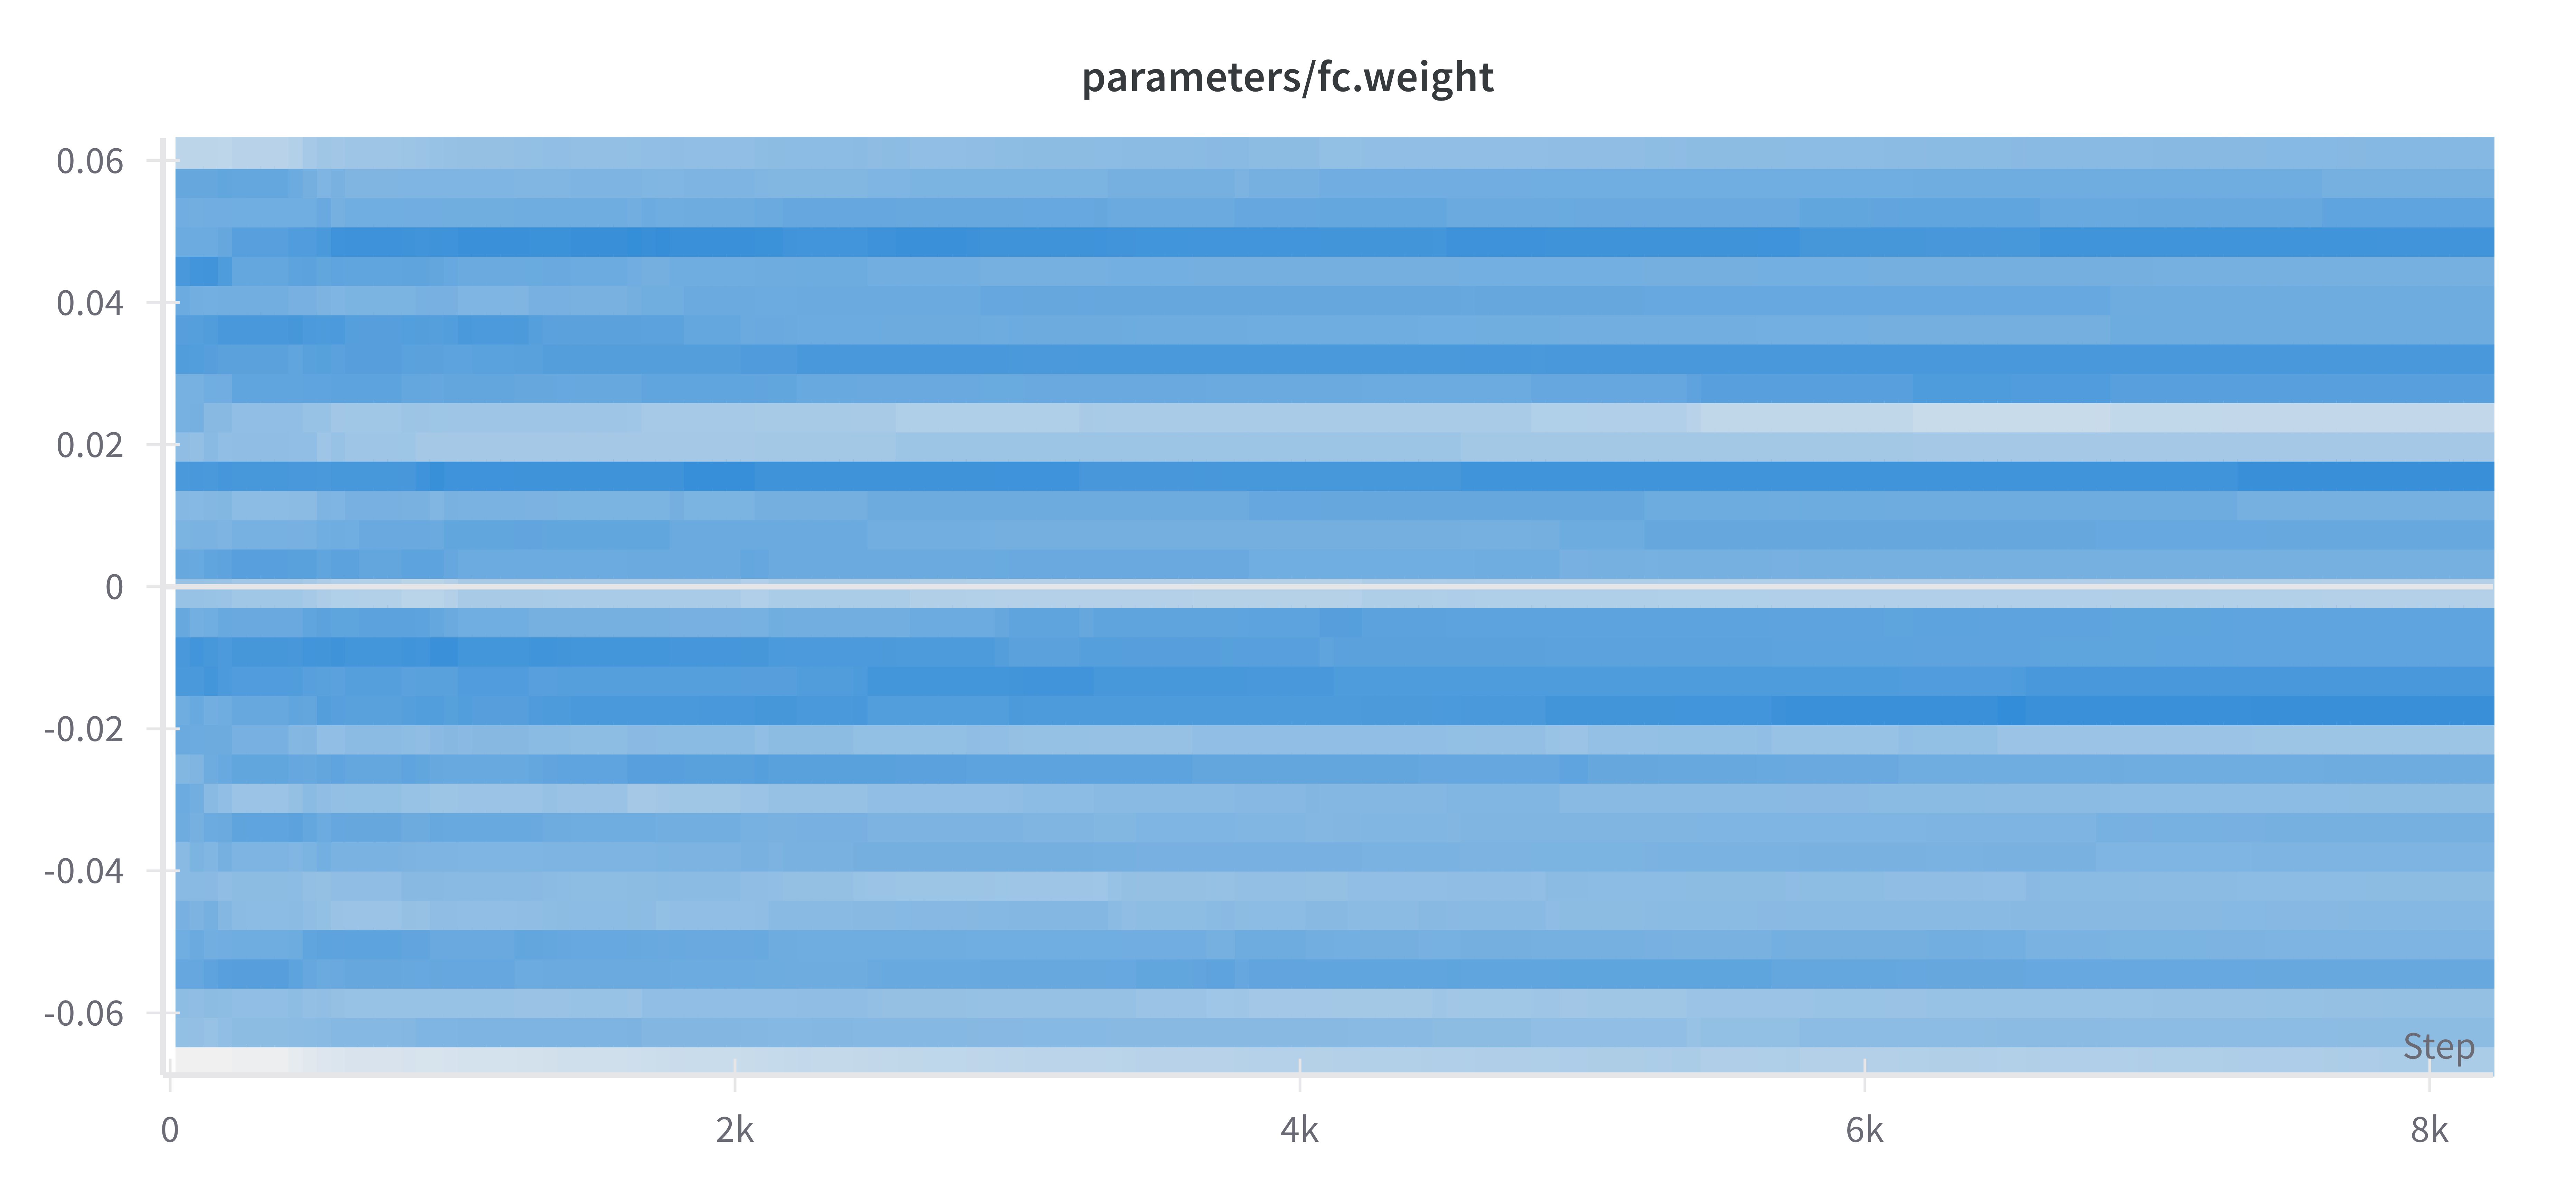
\includegraphics[width=0.7\linewidth]{docs/figs/fc_weights.png}
    \caption{Fully-connected layer weights (Bidirectionally-masked Transformer)}
    \label{fig:fc-weights}
\end{figure}

In Figure~\ref{fig:fc-weights}, we present the weights of the fully connected layer from the model used in Experiment 1 (Table~\ref{table:transformer_model_archs}) across training, validation, and testing. The figure illustrates how the weights of the fully connected layer evolve during training—essentially presenting a top-down view of a histogram. If we were to take vertical slices from this figure, we would get a traditional histogram of the weights at training step $i$.

Since we do not see any significant changes during the training process, we hypothesize the model is not relying heavily on this component to refine or adjust its internal representations over time. If this were to be the case, we would be able to visualize a meaningful pattern or shift in weight values, to correlate with the model learning features from the data. In this case, however, the weights remain nearly static throughout, implying the model is much more reliant on other mechanisms, such as self-attention, rather than the fully connected layer. Consequently, visualizing this layer provides little information regarding explainability or interpretability, making it minimally useful to analyze to gain insights into the model's decision making process.

\begin{figure}[ht!]
    \centering
    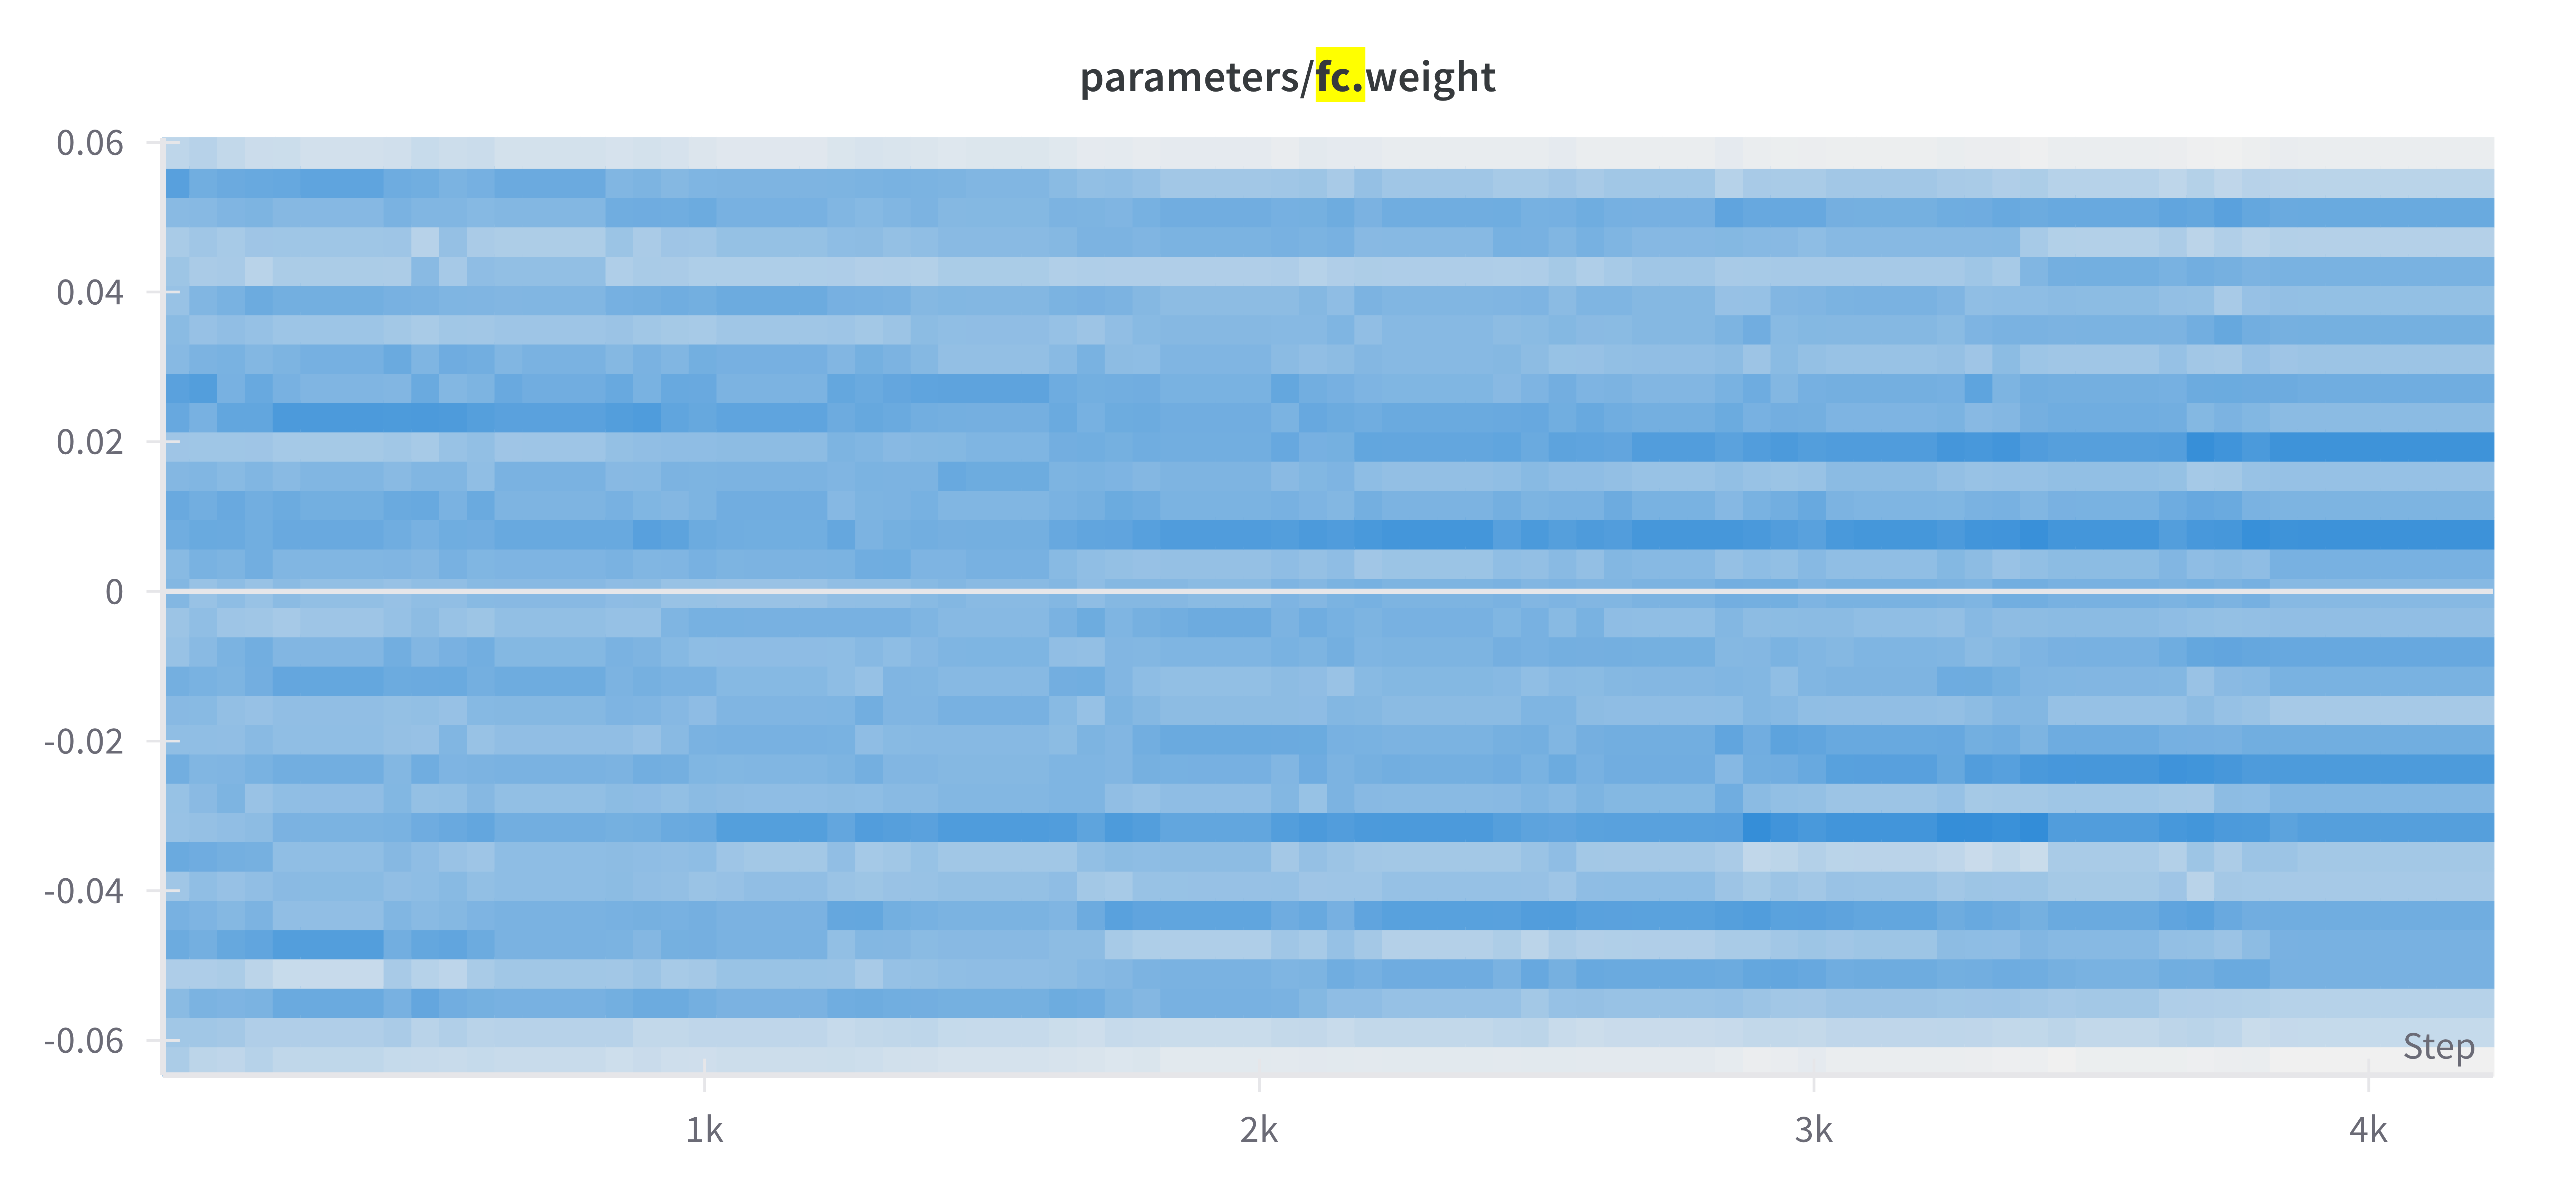
\includegraphics[width=0.7\linewidth]{docs/figs/fc_weights_causal.png}
    \caption{Fully-connected layer weights (Causally-masked Transformer)}
    \label{fig:causal-fc-weights}
\end{figure}

This is supported by the fact that a very similar pattern is observed in the weights of the fully-connected layer of a casually-masked Transformer, as can be seen in Figure~\ref{fig:causal-fc-weights}, leading us to believe that analyzing this component and its weights does not provide information on the model's decision. Instead, it suggests that other components within the model hold more valuable information regarding the model's decision. The fully connected layer appears to function primarily as an output mechanism, mapping the model's internal decisions to a probability distribution.

Our experiments are similar to those carried out by Ebrahimi et al.~\cite{sa-nets-dyck-n}, where they found self-attention networks leverage the attention mechanism to replace the recursion needed to learn hierarchical languages such as Dyck-$k$ with an intelligent representation of the head or start token. In our case, we improved on the performance of self-attention networks to reach perfect accuracy, as detailed in Table~\ref{table:exp_results}. 





